
% Copyright (c) 2015 - 2020 Mario Mlačak, mmlacak@gmail.com
% Public Domain work, under CC0 1.0 Universal Public Domain Dedication. See LICENSING, COPYING files for details.

% Hemera's Dawn chapter ===============================================
\chapter*{Hemera's Dawn}
\addcontentsline{toc}{chapter}{Hemera's Dawn}
\label{ch:Hemera's Dawn}

\begin{flushright}
\parbox{0.8\textwidth}{
\emph{Then assuredly the world was made, not in time, but simultaneously with time. \newline
\hspace*{\fill}{\textperiodcentered \textperiodcentered \textperiodcentered \hspace*{0.2em} St. Augustine} } }
\end{flushright}

\noindent
Hemera's Dawn is chess variant which is played on 20 x 20 board, with
darkish red-brown and grey fields and pure red and bright yellow pieces.
Star colors are bright blue and white.
Three new pieces are introduced; Centaur, Scout, and Grenadier.

\clearpage % ..........................................................
% Centaur *************************************************************

\section*{Centaur}
\addcontentsline{toc}{section}{Centaur}
\label{sec:Hemera's Dawn/Centaur}

\noindent
\begin{wrapfigure}[12]{l}{0.4\textwidth}
\centering
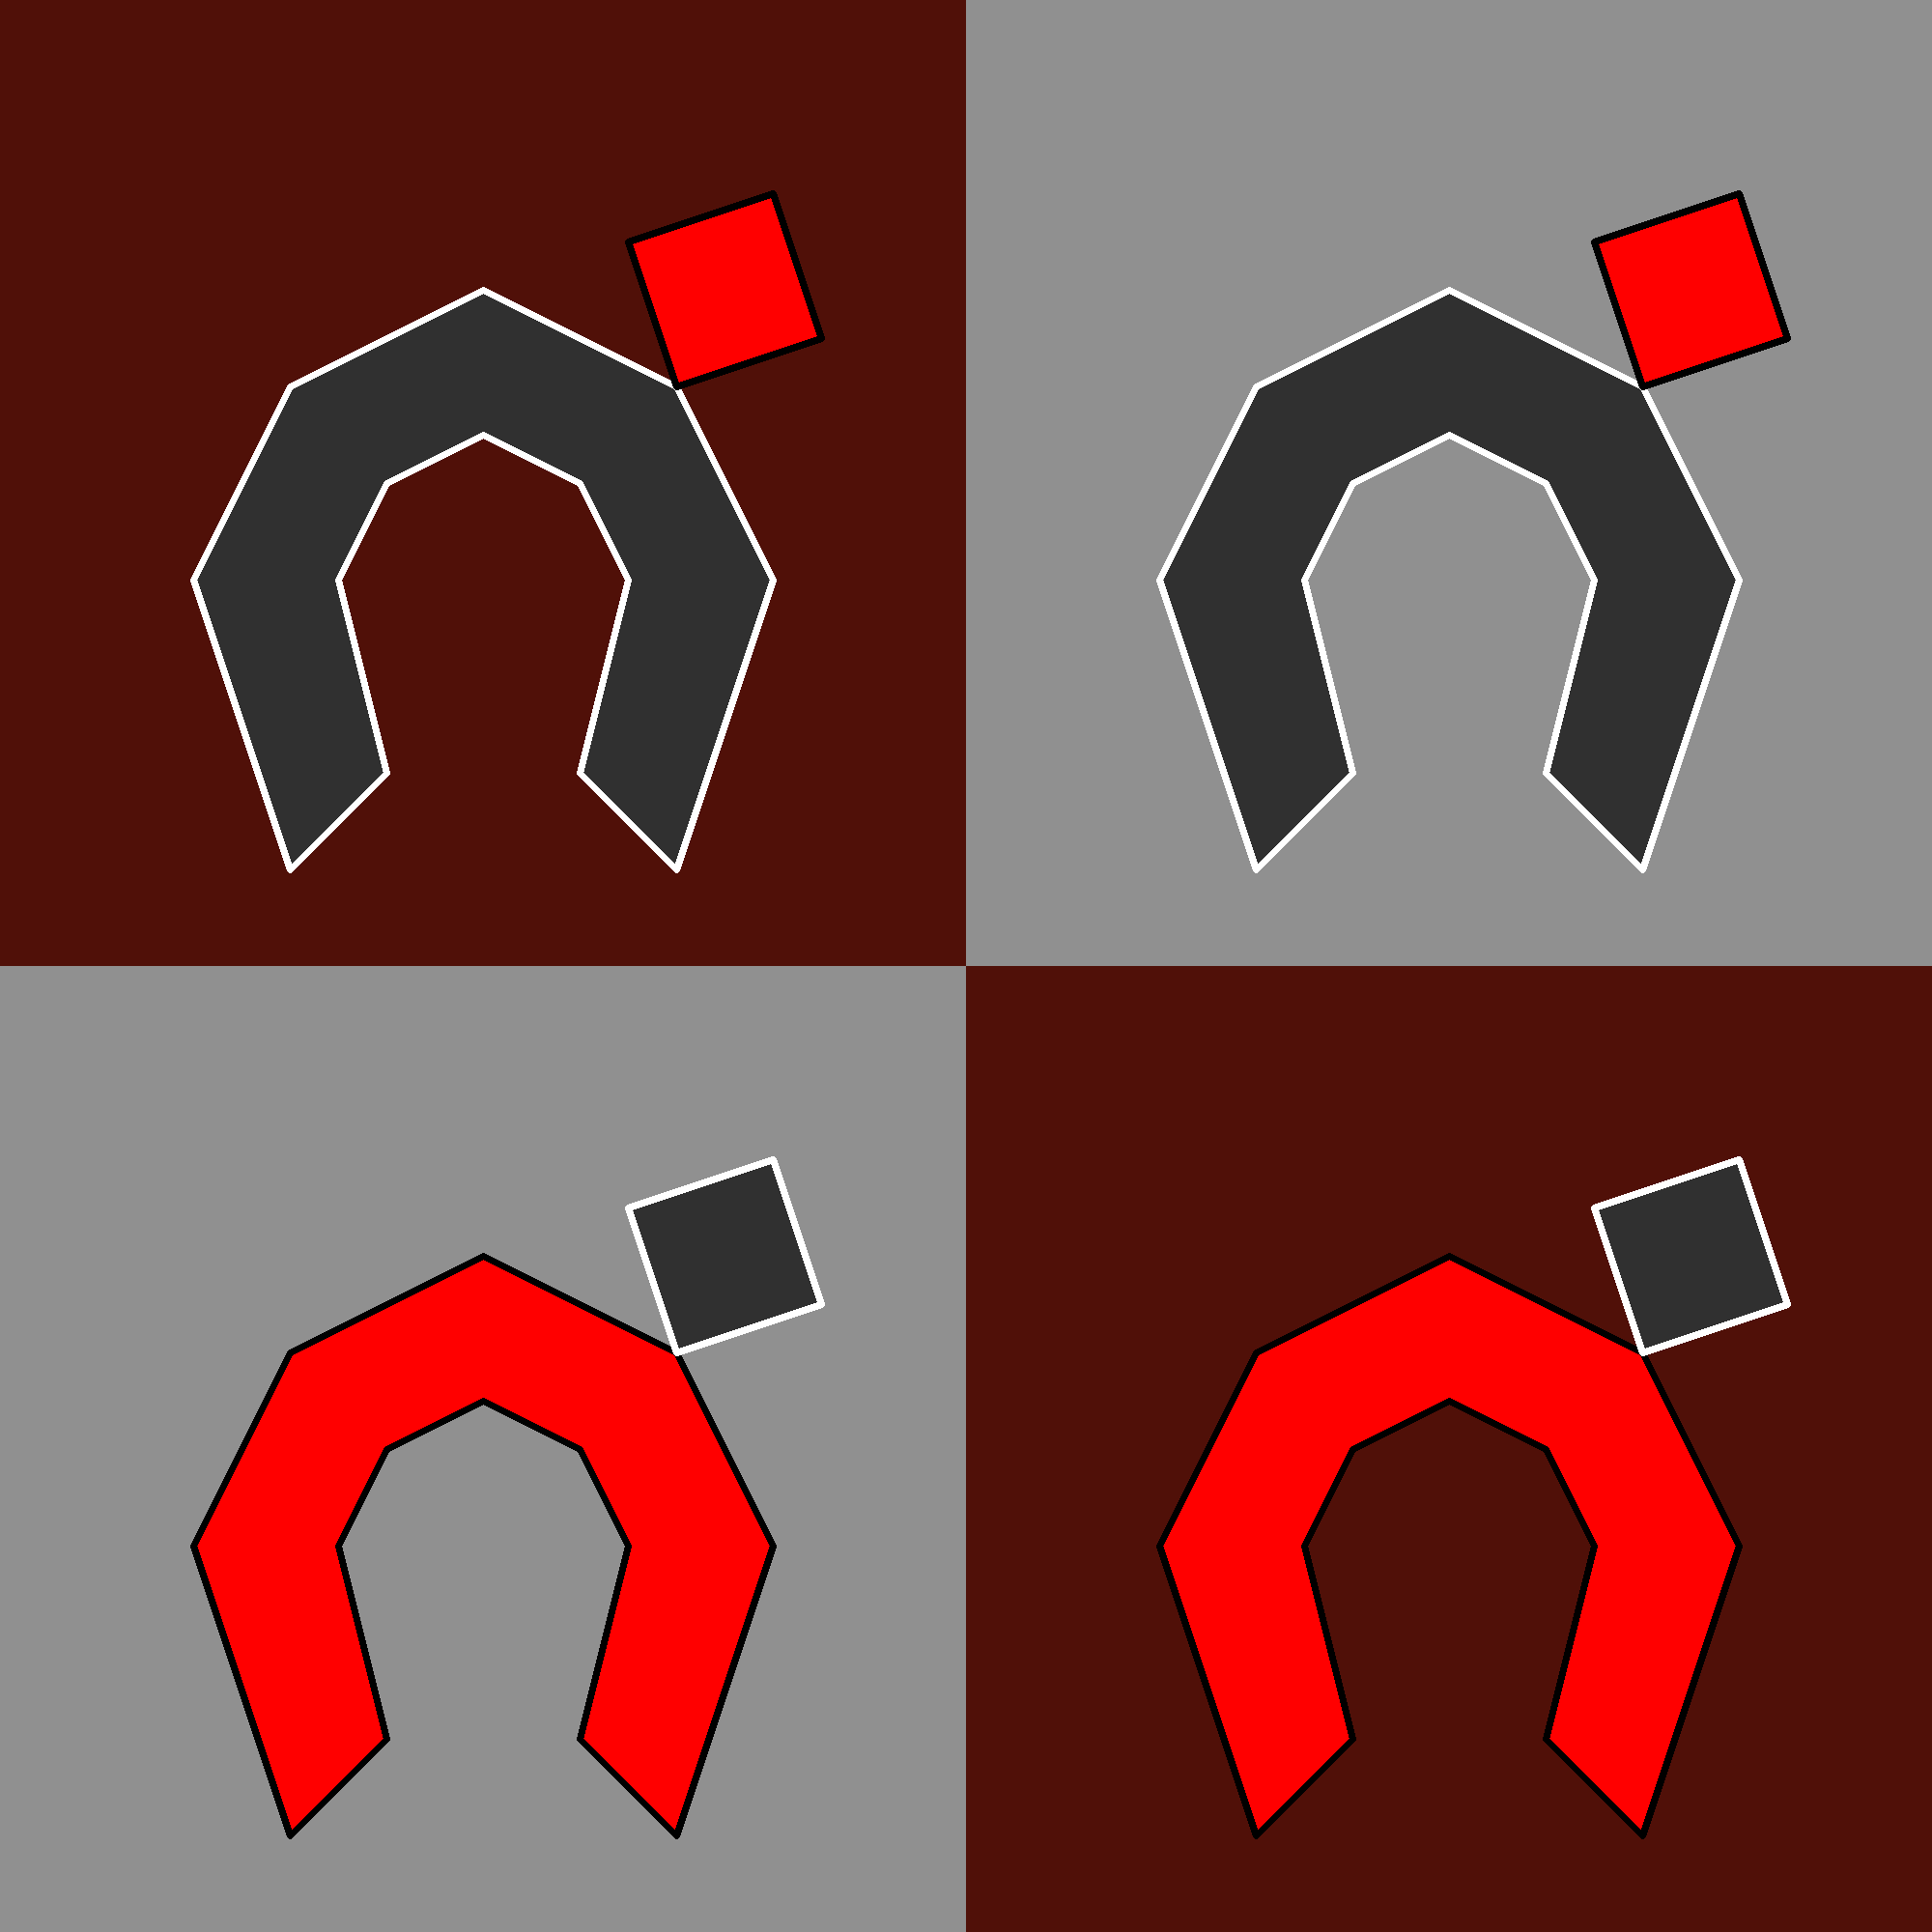
\includegraphics[width=0.4\textwidth, keepaspectratio=true]{pieces/12_centaur.png}
\caption{Centaur}
\label{fig:12_centaur}
\end{wrapfigure}
Centaur is similar to Unicorn, only it can continue its jumpy movement
in two chosen directions until another piece is encountered, or it runs
out of a chessboard.

First direction is chosen freely, second direction is limited by the first
choice. Once both long and short jump directions are determined, Centaur
has to follow them in all subsequent steps, for the remainder of that ply.

For Centaur's ply to be legal, all steps must end up on the chessboard.
Unlike Wave, Centaur cannot step outside of a chessboard, and in later
step(s) return back onto it.

\noindent
\begin{wrapfigure}{l}{0.4\textwidth}
\centering
\includegraphics[width=0.4\textwidth, keepaspectratio=true]{pieces/star/14_hemera_s_dawn.png}
\caption{Star}
\label{fig:star/14_hemera_s_dawn}
\end{wrapfigure}
Star colors in this variant are different to colors of light and dark pieces.

\clearpage % ..........................................................
% Movement ------------------------------------------------------------

% \vspace{7\baselineskip}
\subsection*{Movement}
\addcontentsline{toc}{subsection}{Movement}
\label{sec:Hemera's Dawn/Centaur/Movement}

% \vspace*{-1.1\baselineskip}
\vspace*{-0.7\baselineskip}
\noindent
\begin{minipage}{\textwidth}
\begin{wrapfigure}[9]{l}{0.4\textwidth}
\centering
\includegraphics[width=0.35\textwidth, keepaspectratio=true]{examples/14_hd/scn_hd_01_centaur_same_color.png}
\vspace*{-0.7\baselineskip}
\caption{Centaur short jump}
\label{fig:scn_hd_01_centaur_same_color}
\end{wrapfigure}
On fields with the same color as Centaur, it has the same step-fields (green, blue)
as Knight has.

\mbox{}\newline % Forcing new paragraph ...
On fields in opposite color, Centaur can jump much longer, and has the same step-fields
(green, blue) as Unicorn has. For comparison, short steps are also numbered (grey).
\end{minipage}

\vspace*{0.9\baselineskip}
\noindent
\begin{minipage}{\textwidth}
\begin{wrapfigure}[14]{l}{0.6\textwidth}
\centering
\includegraphics[width=0.55\textwidth, keepaspectratio=true]{examples/14_hd/scn_hd_02_centaur_opposite_color.png}
\vspace*{-0.7\baselineskip}
\caption{Centaur long jump}
\label{fig:scn_hd_02_centaur_opposite_color}
\end{wrapfigure}
Again, just as Knight (and Unicorn), Centaur is not hampered by a piece on any
unmarked field.

\mbox{}\newline % Forcing new paragraph ...
Step-fields are also capture-fields, Centaur would be able to capture opponent's
pieces on any marked field, regardless of marker color (green, blue).
\end{minipage}

\vspace*{0.7\baselineskip}
On initial step, Centaur can freely choose any marked field, regardless of marker
color (green, blue), or step (long, short). On second step, Centaur can choose any
step-field in the other color (blue if green was chosen initially, green if blue
was first choice). On all subsequent steps, Centaur has to keep alternating between
the two initially chosen steps, for the remainder of a ply.

\clearpage % ..........................................................

\noindent
\begin{figure}[!h]
\includegraphics[width=1.0\textwidth, keepaspectratio=true]{examples/14_hd/scn_hd_03_centaur_multi_step_init.png}
\caption{Centaur initial step}
\label{fig:scn_hd_03_centaur_multi_step_init}
\end{figure}

Here, light Centaur is located on the same color (i.e. light) field, so all available
step-fields are short jumps, which are the same as those of Knight. For the first step,
Centaur can choose any of marked step-fields, except the one which is blocked by own
piece (light Pawn).

\clearpage % ..........................................................

\noindent
\begin{figure}[!h]
\includegraphics[width=1.0\textwidth, keepaspectratio=true]{examples/14_hd/scn_hd_04_centaur_multi_step_second.png}
\caption{Centaur second step}
\label{fig:scn_hd_04_centaur_multi_step_second}
\end{figure}

Here, after first step, light Centaur is located on a dark field, so all available
step-fields are long jumps, which are the same as those of Unicorn. Since upper-left
step-field (blue) was chosen for a first step, next step has to be one of upper-right,
lower-left fields (green). Note, opponent's piece (dark Pawn) can be captured, but it
blocks light Centaur from moving any further.

\clearpage % ..........................................................

\noindent
\begin{figure}[!h]
\includegraphics[width=1.0\textwidth, keepaspectratio=true]{examples/14_hd/scn_hd_05_centaur_multi_step.png}
\caption{Centaur complete move}
\label{fig:scn_hd_05_centaur_multi_step}
\end{figure}

After second step is chosen, complete movement of Centaur consists of alternating
between the two initial steps. Centaur for the rest of a ply has to follow those two
initial steps, e.g. after reaching field 6, it cannot move to any other step-field
(red). Light Centaur could also capture dark Bishop, but is prevented from moving
any further (grey). Pieces on all other fields are ignored (Pawns).

\clearpage % ..........................................................

\subsubsection*{Out of board steps}
\addcontentsline{toc}{subsubsection}{Out of board steps}
\label{sec:Hemera's Dawn/Centaur/Movement/Out of board steps}

% \vspace*{-0.05\textwidth}
\vspace*{-1.3\baselineskip}
\noindent
\begin{figure}[!h]
\includegraphics[width=1.0\textwidth, keepaspectratio=true]{examples/14_hd/scn_hd_06_centaur_off_board.png}
\caption{Centaur off-board steps}
\label{fig:scn_hd_06_centaur_off_board}
\end{figure}

Here, light grey fields are virtual fields extending existing chessboard. For
Centaur, it's illegal to step outside of a chessboard, and all subsequent steps
are also illegal.

Here, Centaur cannot reach fields 1 and 2 from starting position with selected
directions, even though it would end movement on the chessboard.

% ------------------------------------------------------------ Movement
\clearpage % ..........................................................
% Activating Wave -----------------------------------------------------

\subsection*{Activating Wave}
\addcontentsline{toc}{subsection}{Activating Wave}
\label{sec:Hemera's Dawn/Centaur/Activating Wave}

\vspace*{-1.3\baselineskip}
\noindent
\begin{figure}[!h]
\includegraphics[width=1.0\textwidth, keepaspectratio=true]{examples/14_hd/scn_hd_07_wave_activation_by_centaur_first_step.png}
\caption{Wave activation by Centaur, first step}
\label{fig:scn_hd_07_wave_activation_by_centaur_first_step}
\end{figure}

Wave activated by Centaur, \hyperref[fig:scn_hd_01_centaur_same_color]{moves like one}.
Here, light Wave is activated on the opposite color (i.e. dark) field, so all available
step-fields are long jumps, which are the same as those of Unicorn. For the first step,
Wave can choose any of marked step-fields (green, blue), including the one occupied by
own piece (light Pawn). Light Pawn could be activated, or stepped over.

\clearpage % ..........................................................

% \vspace*{-1.0\baselineskip}
\noindent
\begin{figure}[!h]
\includegraphics[width=1.0\textwidth, keepaspectratio=true]{examples/14_hd/scn_hd_08_wave_activation_by_centaur_second_step.png}
\caption{Wave activation by Centaur, second step}
\label{fig:scn_hd_08_wave_activation_by_centaur_second_step}
\end{figure}

After first step, light Wave is located on a light field, so all available step-fields
are short jumps, which are the same as those of Knight. Since upper-right step-field
(green) was chosen for a first step, next step has to be one of upper-left, lower-right
fields (blue). Light Wave cannot activate opponent's piece (dark Pawn), but it can step
over it.

\clearpage % ..........................................................

% \vspace*{-1.0\baselineskip}
\noindent
\begin{figure}[!h]
\includegraphics[width=1.0\textwidth, keepaspectratio=true]{examples/14_hd/scn_hd_09_wave_activation_by_centaur_complete.png}
\caption{Wave activation by Centaur}
\label{fig:scn_hd_09_wave_activation_by_centaur_complete}
\end{figure}

After second step is chosen, complete movement of Wave consists of alternating between
the two initially chosen steps, which Wave for the rest of a ply has to follow, e.g.
after reaching field 4, it cannot move to any other step-field (red). Light Wave could
also activate dark Wave, or it could continue moving further. Pieces on all other fields
are ignored (Pawns).

\clearpage % ..........................................................

\subsubsection*{Out of board steps}
\addcontentsline{toc}{subsubsection}{Out of board steps}
\label{sec:Hemera's Dawn/Centaur/Activating Wave/Out of board steps}

\vspace*{-1.2\baselineskip}
\noindent
\begin{figure}[!h]
\includegraphics[width=1.0\textwidth, keepaspectratio=true]{examples/14_hd/scn_hd_10_wave_activated_by_centaur_off_board.png}
\caption{Wave off-board steps}
\label{fig:scn_hd_10_wave_activated_by_centaur_off_board}
\end{figure}

Again, light grey fields are virtual fields extending existing chessboard.
Wave activated by Centaur can step outside of a board, as long as its ply
ends on a board, just like
\hyperref[fig:scn_mv_30_wave_off_board]{Wave activated by Unicorn}. Here,
step-fields 1 and 2 are reachable by Wave, even though it stepped outside
of the board. It is illegal for any piece, including Wave, to end its ply
outside of a board.

\clearpage % ..........................................................

\subsection*{Teleporting Wave}
\addcontentsline{toc}{subsection}{Teleporting Wave}
\label{sec:Hemera's Dawn/Centaur/Teleporting Wave}

\vspace*{-1.2\baselineskip}
\noindent
\begin{figure}[!h]
\includegraphics[width=1.0\textwidth, keepaspectratio=true]{examples/14_hd/scn_hd_11_wave_teleport.png}
\caption{Wave off-board teleporting}
\label{fig:scn_hd_11_wave_teleport}
\end{figure}

Activation by Centaur and following teleportation of Wave is
\hyperref[fig:scn_n_07_teleport_wave_init]{exactly the same as if activated by Unicorn},
except Wave can now carry more than 1 momentum, because Centaur's ply can be
longer than just 1 step.

% ----------------------------------------------------- Activating Wave
% ************************************************************* Centaur
\clearpage % ..........................................................
% Scout ***************************************************************

\section*{Scout}
\addcontentsline{toc}{section}{Scout}
\label{sec:Hemera's Dawn/Scout}

\vspace*{-0.7\baselineskip}
\noindent
\begin{wrapfigure}[9]{l}{0.4\textwidth}
\centering
\includegraphics[width=0.4\textwidth, keepaspectratio=true]{pieces/13_scout.png}
\vspace*{-1.3\baselineskip}
\caption{Scout}
\label{fig:13_scout}
\end{wrapfigure}
Scout is more mobile relative of a Pawn. Like Pawn, Scout can rush, and can be captured
by en passant. Also like Pawn, Scout can capture opponent's rushing privates (Pawns,
Scouts, Grenadiers) by en passant. Unlike Pawn, Scout cannot be promoted. Pawns can be
promoted to Scouts.

\vspace*{0.7\baselineskip}
\subsection*{Movement}
\addcontentsline{toc}{subsection}{Movement}
\label{sec:Hemera's Dawn/Scout/Movement}

\vspace*{-1.3\baselineskip}
\noindent
\begin{figure}[!h]
\includegraphics[width=1.0\textwidth, keepaspectratio=true]{examples/14_hd/scn_hd_15_scout_movement.png}
\vspace*{-1.3\baselineskip}
\caption{Scout movement}
\label{fig:scn_hd_15_scout_movement}
\end{figure}

\vspace*{-0.5\baselineskip}
Scout can make a few steps forward (towards opponent's initial positions), and
to the sides. Forward movement is the same as Pawn's; light Scout moves straight
upwards, while dark Scout moves straight downwards. Count of steps Scout can make
depends on size of a chessboard; in this variant Scout can make up to 5 steps in
each direction.

\clearpage % ..........................................................

Scout can also capture opponent's pieces with its diagonal steps; unlike Pawn's,
those are backwards steps, i.e. towards own initial positions. \newline
\indent
Steps (arrows) are referred to by relative position of its end field (point).
So, capture-steps for light Scout are down-left, down-right diagonals;
and for dark Scout up-left, up-right diagonals.

\vspace*{-0.3\baselineskip}
\noindent
\begin{wrapfigure}[7]{l}{0.41\textwidth}
\centering
\includegraphics[width=0.4\textwidth, keepaspectratio=true]{examples/14_hd/scn_hd_16_scout_capturing.png}
\vspace*{-0.3\baselineskip}
\caption{Scout capturing}
\label{fig:scn_hd_16_scout_capturing}
\end{wrapfigure}
Like Pawn, Scout can capture only on its first step in a ply, and cannot capture
after it started moving. Here, light Scout can capture dark Knight since it's
first step, but cannot capture dark Bishop after it made 3 steps to the right.

% \TODO :: fix lmodern

\vspace*{-0.7\baselineskip}
\subsubsection*{Forking steps}
\addcontentsline{toc}{subsubsection}{Forking steps}
\label{sec:Hemera's Dawn/Scout/Movement/Forking steps}

\vspace*{-0.7\baselineskip}
\noindent
\begin{wrapfigure}[14]{l}{0.4\textwidth}
\centering
\includegraphics[width=0.35\textwidth, keepaspectratio=true]{examples/14_hd/scn_hd_17_scout_forking_steps.png}
\vspace*{-0.3\baselineskip}
\caption{Forking steps}
\label{fig:scn_hd_17_scout_forking_steps}
\end{wrapfigure}
Forking steps refer to two diagonal steps available after a step up, down, left
or right is made. \newline
\indent
Forked steps are extension of a first step; so, e.g. after left step only left-up,
and left-down steps are available, but not right-up, right-down. \newline
\indent
Here are shown all forking steps for both light and dark Scout. Light Scout would
use forking step after left, up, or right steps are taken; dark Scout would chose
forking step after left, down, or right steps.

\clearpage % ..........................................................

\subsubsection*{Rerouting Scout}
\addcontentsline{toc}{subsubsection}{Rerouting Scout}
\label{sec:Hemera's Dawn/Scout/Movement/Rerouting Scout}

% \TODO :: fix lmodern

\vspace*{-0.7\baselineskip}
\noindent
\begin{wrapfigure}[9]{l}{0.41\textwidth}
\centering
\includegraphics[width=0.4\textwidth, keepaspectratio=true]{examples/14_hd/scn_hd_20_scout_rerouting.png}
\vspace*{-0.3\baselineskip}
\caption{Rerouting Scout}
\label{fig:scn_hd_20_scout_rerouting}
\end{wrapfigure}
Scout's horizontal and vertical steps are just a movement steps, and so can be blocked.
When step is blocked, Scout can choose one of associated diagonal, forking step to
move around obstacle. Then, Scout has to continue its movement in the same direction
it was moving before rerouting.

\vspace*{-0.7\baselineskip}
\noindent
\begin{wrapfigure}[9]{l}{0.41\textwidth}
\centering
\includegraphics[width=0.4\textwidth, keepaspectratio=true]{examples/14_hd/scn_hd_21_scout_rerouting_first_step.png}
\vspace*{-0.3\baselineskip}
\caption{Rerouting first step}
\label{fig:scn_hd_21_scout_rerouting_first_step}
\end{wrapfigure}
\indent
In rerouting examples here blue arrows are used just to distinguish one valid path over
the other, when choice (forking step) is being made. \newline
\indent
First step can also be blocked (including by own piece), direction to follow after
rerouting is the blocked one.

\vspace*{-0.7\baselineskip}
\noindent
\begin{wrapfigure}[11]{l}{0.41\textwidth} % 10 = enough
\centering
\includegraphics[width=0.4\textwidth, keepaspectratio=true]{examples/14_hd/scn_hd_22_scout_rerouting_pawn_wall.png}
\vspace*{-0.3\baselineskip}
\caption{Continuous rerouting}
\label{fig:scn_hd_22_scout_rerouting_pawn_wall}
\end{wrapfigure}
\indent
If initially chosen direction is blocked after rerouting, Scout can be rerouted
again. Each choice of forking step is independent from any previous choice. \newline
\indent
Here, each time Scout is blocked by any Pawn (own or opponent's), it can choose
between equally valid right-down or right-up forking steps, regardless of any
previous choices.

\clearpage % ..........................................................

\subsection*{Activating Scout}
\addcontentsline{toc}{subsection}{Activating Scout}
\label{sec:Hemera's Dawn/Scout/Activating Scout}

\vspace*{-1.3\baselineskip}
\noindent
\begin{figure}[!h]
\includegraphics[width=1.0\textwidth, keepaspectratio=true]{examples/14_hd/scn_hd_23_activating_scout.png}
\vspace*{-1.3\baselineskip}
\caption{Activating Scout}
\label{fig:scn_hd_23_activating_scout}
\end{figure}

\vspace*{-0.5\baselineskip}
Activated Scout is limited by both count of steps it can make, and momentum it
received, whichever is lower. In this variant, Scout can make at most 5 steps;
limit depends on size of a chessboard. Here, light Scout is activated by own
Queen via Wave. Wave C is out of reach for light Scout, even though it received
11 momentum.

Activated Scout uses received momentum for movement, and transfers all of
remaining momentum to the piece it activates. Here, light Scout can activate
Wave B, and transfer to it remaining 7 momentum.

\clearpage % ..........................................................

\subsection*{Activating Wave, Pyramid}
\addcontentsline{toc}{subsection}{Activating Wave, Pyramid}
\label{sec:Hemera's Dawn/Scout/Activating Wave, Pyramid}

\vspace*{-1.3\baselineskip}
\noindent
\begin{figure}[!h]
\includegraphics[width=1.0\textwidth, keepaspectratio=true]{examples/14_hd/scn_hd_24_scout_activating_wave_step_fields.png}
\vspace*{-1.3\baselineskip}
\caption{Activating Wave on step-fields}
\label{fig:scn_hd_24_scout_activating_wave_step_fields}
\end{figure}

\vspace*{-0.5\baselineskip}
Wave activated by Scout on its step-fields can move left, right, or forward
(towards opponent's initial positions); the same as
\hyperref[fig:scn_n_17_sideways_pawn_activated_wave]{Wave activated by Pawn on its step-field}.
Direction, once chosen, cannot be changed for duration of a ply. Activated
Wave is not limited by received momentum, and so can move until end of a
chessboard is reached. Wave activated on step-fields cannot activate Pyramid.

\hyperref[fig:scn_n_18_sideways_pawn_does_not_activate_pyramid]{The same as Pawn},
Scout cannot activate Pyramid on its step-fields, neither directly nor indirectly
(via Wave).

\clearpage % ..........................................................

\vspace*{-2.3\baselineskip}
\noindent
\begin{figure}[!h]
\includegraphics[width=1.0\textwidth, keepaspectratio=true]{examples/14_hd/scn_hd_25_scout_activating_wave_capture_fields.png}
\vspace*{-1.3\baselineskip}
\caption{Activating Wave on capture-fields}
\label{fig:scn_hd_25_scout_activating_wave_capture_fields}
\end{figure}

\vspace*{-0.5\baselineskip}
Wave activated by Scout on its capture-fields can move diagonally left or right,
towards own initial positions. This is similar to
\hyperref[fig:scn_mv_23_wave_activation_by_capture_pawn]{Wave activated by Pawn on its capture-field},
except Wave steps are now backwards. Direction, once chosen, cannot be changed for
duration of a ply. Activated Wave is not limited by received momentum, and so can
move until end of a chessboard is reached. Wave activated on a capture-field can
activate a Pyramid.

Scout can activate Pyramid on its capture-fields. Cascade in which Pyramid is
activated can contain Scout moving over its step-fields, as long as last material
(non-Wave) piece is the one which can activate Pyramid; this is
\hyperref[fig:scn_n_19_sideways_pawns_cascade_pyramids]{the same as in cascade with a Pawn}.

\clearpage % ..........................................................

\subsection*{En passant}
\addcontentsline{toc}{subsection}{En passant}
\label{sec:Hemera's Dawn/Scout/En passant}

\vspace*{-0.7\baselineskip}
\noindent
\begin{wrapfigure}[14]{l}{0.4\textwidth}
\centering
\includegraphics[width=0.25\textwidth, keepaspectratio=true]{examples/14_hd/scn_hd_26_scout_en_passant.png}
\vspace*{-0.3\baselineskip}
\caption{En passant}
\label{fig:scn_hd_26_scout_en_passant}
\end{wrapfigure}
\indent
In this, and all subsequent variants, any private (Pawn, Scout, or Grenadier) can
capture any other opponent's private en passant; types of pieces do not need to
match. \newline
\indent
For example, light Scout could capture rushing dark Grenadier en passant, just as
Pawns are able to do the same to rushing opponent's Pawns in Classical Chess.

Capturing rushing opponent's Pawn with Scout is very similar to
\href{https://en.wikipedia.org/wiki/En_passant}{en passant with a Pawn},
the only real difference is that Pawn captures at forward, diagonal field,
i.e. towards opponent's initial positions, while Scout captures at diagonal
field backwards, i.e. towards own initial positions.

Here, dark Scout and dark Pawn are both positioned on the same rank, and both
can capture rushing light Pawn en passant; the only difference between capturing
with either of those two pieces are their capture-fields.

\clearpage % ..........................................................

\subsection*{Initial positions}
\addcontentsline{toc}{subsection}{Initial positions}
\label{sec:Hemera's Dawn/Scout/Initial positions}

\vspace*{-1.2\baselineskip}
\noindent
\begin{figure}[!h]
\includegraphics[width=1.0\textwidth, keepaspectratio=true]{examples/14_hd/scn_hd_39_scout_initial_positions.png}
\vspace*{-1.3\baselineskip}
\caption{Initial positions of Scouts}
\label{fig:scn_hd_39_scout_initial_positions}
\end{figure}

\vspace*{-0.5\baselineskip}
In this variant a set of Scouts are added to
\hyperref[fig:14_hemera_s_dawn]{the initial setup}, 8 to each light and dark
player, in front of regular Pawn ranks.

Scouts are positioned relative to Centaurs' initial positions, to block them
from capturing opponent's pieces from the very first move.

% *************************************************************** Scout
\clearpage % ..........................................................
% Grenadier ***********************************************************

\section*{Grenadier}
\addcontentsline{toc}{section}{Grenadier}
\label{sec:Hemera's Dawn/Grenadier}

\vspace*{-0.7\baselineskip}
\noindent
\begin{wrapfigure}[10]{l}{0.4\textwidth}
\centering
\includegraphics[width=0.4\textwidth, keepaspectratio=true]{pieces/14_grenadier.png}
\vspace*{-1.3\baselineskip}
\caption{Grenadier}
\label{fig:14_grenadier}
\end{wrapfigure}
Grenadier is more tactical relative of a Pawn. Like Pawn, Grenadier can rush, and
can be captured by en passant. Also like Pawn, Grenadier can capture opponent's
rushing privates (Pawns, Scouts, Grenadiers) by en passant. Unlike Pawn, Grenadier
cannot be promoted. Pawns can be promoted to Grenadiers.

% \TODO :: fix lmodern

\vspace*{-0.3\baselineskip}
\subsection*{Grenadier-fields}
\addcontentsline{toc}{subsection}{Grenadier-fields}
\label{sec:Hemera's Dawn/Grenadier/Grenadier-fields}

\vspace*{-0.7\baselineskip}
\noindent
\begin{wrapfigure}[9]{l}{0.4\textwidth}
\centering
\includegraphics[width=0.25\textwidth, keepaspectratio=true]{examples/14_hd/scn_hd_40_grenadier_fields.png}
\vspace*{-0.5\baselineskip}
\caption{Grenadier-fields}
\label{fig:scn_hd_40_grenadier_fields}
\end{wrapfigure}
Grenadier-fields are all fields immediately neighboring Grenadier horizontally,
vertically, and diagonally. They are the same fields as step-fields of a King. \newline
\indent
Grenadier is in close quarters if there is at least one opponent's piece present
on its grenadier-fields.

\vspace*{-1.7\baselineskip}
\subsection*{Movement}
\addcontentsline{toc}{subsection}{Movement}
\label{sec:Hemera's Dawn/Grenadier/Movement}

\vspace*{-0.7\baselineskip}
Light and dark Grenadier moves in the same way; so, in following examples only
light Grenadier movement is shown. \newline
\indent
When starting a ply Grenadier can move to, and capture at different fields
depending if it's in close quarters or not. \newline
\indent
Just like Pawn, Grenadier have capture- and step-fields separated, and so it
can move onto capture-field only if there is opponent's piece to be captured.

\clearpage % ..........................................................

\vspace*{-1.7\baselineskip}
\noindent
\begin{wrapfigure}[9]{l}{0.4\textwidth}
\centering
\includegraphics[width=0.39\textwidth, keepaspectratio=true]{examples/14_hd/scn_hd_41_grenadier_movement.png}
\vspace*{-0.5\baselineskip}
\caption{Movement}
\label{fig:scn_hd_41_grenadier_movement}
\end{wrapfigure}
When there is no opponent's piece on its grenadier-field, Grenadier can take up
to 3 fields to the left or right, and at most 2 fields up or down; these are
step-fields, so e.g. Pyramid cannot be activated on them (green arrows). Movement
limits depends on size of a chessboard. \newline
\indent
Grenadier can capture only at closest neighboring fields at all 4 diagonals (red
arrows).

% \TODO :: fix lmodern

\vspace*{-0.7\baselineskip}
\noindent
\begin{wrapfigure}[6]{l}{0.4\textwidth}
\centering
\includegraphics[width=0.35\textwidth, keepaspectratio=true]{examples/14_hd/scn_hd_42_grenadier_movement_transition.png}
\vspace*{-0.5\baselineskip}
\caption{Transition}
\label{fig:scn_hd_42_grenadier_movement_transition}
\end{wrapfigure}
Presence of opponent's pieces on grenadier-fields is relevant only at the start of
Grenadier's ply. \newline
\indent
So, Grenadier which started a ply without opponent's piece on its grenadier-fields
won't gain (or lose) any steps, if it passes by opponent's piece.

\vspace*{-1.3\baselineskip}
\subsubsection*{Forking steps}
\addcontentsline{toc}{subsubsection}{Forking steps}
\label{sec:Hemera's Dawn/Grenadier/Movement/Forking steps}

\vspace*{-0.7\baselineskip}
\noindent
\begin{wrapfigure}[11]{l}{0.4\textwidth}
\centering
\includegraphics[width=0.35\textwidth, keepaspectratio=true]{examples/14_hd/scn_hd_43_forking_steps.png}
\vspace*{-0.5\baselineskip}
\caption{Forking steps}
\label{fig:scn_hd_43_forking_steps}
\end{wrapfigure}
Forking steps refer to two diagonal capture-steps available after a step up, down,
left or right is made. \newline
\indent
Steps (arrows) are referred to by relative position of its end point. \newline
\indent
Forked capture-steps available are extension of first step; so, e.g. after left
step only left-up, and left-down capture-steps are available, but not right-up,
right-down. \newline
\indent
Here, all possible choices for first step followed by its accompanying
capture-steps are shown.

\clearpage % ..........................................................

\subsubsection*{Close quarters}
\addcontentsline{toc}{subsubsection}{Close quarters}
\label{sec:Hemera's Dawn/Grenadier/Movement/Close quarters}

\vspace*{-0.7\baselineskip}
\noindent
\begin{wrapfigure}[10]{l}{0.4\textwidth}
\centering
\includegraphics[width=0.25\textwidth, keepaspectratio=true]{examples/14_hd/scn_hd_44_grenadier_vertical_steps.png}
\vspace*{-0.5\baselineskip}
\caption{Vertical steps}
\label{fig:scn_hd_44_grenadier_vertical_steps}
\end{wrapfigure}
When there is opponent's piece on its grenadier-fields, Grenadier can take one step
up or down; after which it can take associated forking capture-step, if there is
opponent's piece to capture (here, dark Bishop). Before taking any other step,
Grenadier can take diagonal capture-step; here, capturing dark Knight.

\vspace*{-0.7\baselineskip}
\noindent
\begin{figure}[!h]
\includegraphics[width=1.0\textwidth, keepaspectratio=true]{examples/14_hd/scn_hd_45_grenadier_horizontal_steps.png}
\vspace*{-1.4\baselineskip}
\caption{Horizontal steps}
\label{fig:scn_hd_45_grenadier_horizontal_steps}
\end{figure}

\vspace*{-0.7\baselineskip}
In close quarters, Grenadier can take one step more than count of opponent's pieces
on its grenadier-fields either to the left or to the right; here, three opponent's
pieces grants four horizontal steps. After each step Grenadier can optionally capture
opponent's piece with associated forked capture-step (here, dark Queen).

\vspace*{-0.7\baselineskip}
\noindent
\begin{wrapfigure}[6]{l}{0.4\textwidth}
\centering
\includegraphics[width=0.35\textwidth, keepaspectratio=true]{examples/14_hd/scn_hd_46_grenadier_close_quarters_transition.png}
\vspace*{-0.5\baselineskip}
\caption{Transition}
\label{fig:scn_hd_46_grenadier_close_quarters_transition}
\end{wrapfigure}
\hyperref[fig:scn_hd_42_grenadier_movement_transition]{Again},
whether Grenadier is in close quarters is determined at the very beginning of a ply,
before first step; and also how many steps it's being granted due to opponent's pieces
on its grenadier-fields. \newline
% \indent
Here, Grenadier after first step has no opponent's pieces in its vicinity, yet it
still can capture dark Queen.

\clearpage % ..........................................................

\vspace*{-1.7\baselineskip}
\noindent
\begin{wrapfigure}[4]{l}{0.41\textwidth}
\centering
\includegraphics[width=0.4\textwidth, keepaspectratio=true]{examples/14_hd/scn_hd_47_grenadier_blocked_steps.png}
\vspace*{-0.5\baselineskip}
\caption{Blocked steps}
\label{fig:scn_hd_47_grenadier_blocked_steps}
\end{wrapfigure}
Grenadier cannot capture on its step-fields, so those can be blocked, and with it
all subsequent step- and forked capture-fields.

% \TODO :: fix lmodern

\vspace*{2.3\baselineskip}
\noindent
\begin{wrapfigure}[5]{l}{0.41\textwidth}
\centering
\includegraphics[width=0.4\textwidth, keepaspectratio=true]{examples/14_hd/scn_hd_48_grenadier_not_blocked_steps.png}
\vspace*{-0.5\baselineskip}
\caption{Steps not blocked}
\label{fig:scn_hd_48_grenadier_not_blocked_steps}
\end{wrapfigure}
\hyperref[fig:scn_mv_07_wave_is_transparent]{Waves are transparent}, so do not block
subsequent fields. Grenadier cannot interact with opponent's Wave, so that step-field
is blocked, but not fields behind it.

\vspace*{1.0\baselineskip}
\noindent
\begin{figure}[!h]
\includegraphics[width=1.0\textwidth, keepaspectratio=true]{examples/14_hd/scn_hd_49_grenadier_close_quarters_pattern.png}
\vspace*{-1.3\baselineskip}
\caption{Complete close quarters pattern}
\label{fig:scn_hd_49_grenadier_close_quarters_pattern}
\end{figure}

\vspace*{-0.5\baselineskip}
Steps, normal and forked capture-steps taken together form complete movement pattern
in close quarters, i.e. when opponent's pieces were present on its grenadier-fields,
before Grenadier took first step in a ply. \newline
\indent
Note, in close quarters Grenadier can take only one step up or down; regardless how
many opponent's pieces there are on its grenadier-fields.

\clearpage % ..........................................................

\subsection*{Activating Grenadier}
\addcontentsline{toc}{subsection}{Activating Grenadier}
\label{sec:Hemera's Dawn/Grenadier/Activating Grenadier}

\vspace*{-0.7\baselineskip}
\noindent
\begin{wrapfigure}[7]{l}{0.4\textwidth}
\centering
\includegraphics[width=0.35\textwidth, keepaspectratio=true]{examples/14_hd/scn_hd_50_grenadier_activated.png}
\vspace*{-0.5\baselineskip}
\caption{Activated}
\label{fig:scn_hd_50_grenadier_activated}
\end{wrapfigure}
Activated Grenadier is limited by received momentum, up to maximum allowed by movement
pattern; both in close quarters, and out. Both normal and capture-steps are counted
towards movement limit.

% \TODO :: fix lmodern

\vspace*{-0.7\baselineskip}
\noindent
\begin{figure}[!h]
\includegraphics[width=1.0\textwidth, keepaspectratio=true]{examples/14_hd/scn_hd_51_grenadier_close_quarters_activation.png}
\vspace*{-1.4\baselineskip}
\caption{Activating close quarters Grenadier}
\label{fig:scn_hd_51_grenadier_close_quarters_activation}
\end{figure}

\vspace*{-1.2\baselineskip}
\noindent
\begin{figure}[!h]
\includegraphics[width=1.0\textwidth, keepaspectratio=true]{examples/14_hd/scn_hd_52_grenadier_close_quarters_activated.png}
\vspace*{-1.4\baselineskip}
\caption{Close quarters Grenadier activated}
\label{fig:scn_hd_52_grenadier_close_quarters_activated}
\end{figure}

\vspace*{-0.5\baselineskip}
Here, Grenadier activated in close quarters (now "in the air") cannot capture dark
Queen, since it's limited by received 3 momentum. \newline
\indent
Any surplus momentum is lost, unless Grenadier activates a piece. Just like any
other piece, Grenadier can activate own Wave on either step- or capture-fields,
while own Pyramid can be activated only on capture-fields. As before, all of
remaining momentum is transferred to activated piece.

\clearpage % ..........................................................

\subsection*{Activating Wave, Pyramid}
\addcontentsline{toc}{subsection}{Activating Wave, Pyramid}
\label{sec:Hemera's Dawn/Grenadier/Activating Wave, Pyramid}

\vspace*{-1.1\baselineskip}
\noindent
\begin{wrapfigure}[6]{l}{0.4\textwidth}
\centering
\includegraphics[width=0.25\textwidth, keepaspectratio=true]{examples/14_hd/scn_hd_53_grenadier_activating_wave_step_field.png}
\vspace*{-0.5\baselineskip}
\caption{Activating}
\label{fig:scn_hd_53_grenadier_activating_wave_step_field}
\end{wrapfigure}
Wave activated by Grenadier on its step-fields moves like a Rook, straight to the
left, right, up, or down; regardless if activating Grenadier was in close quarters,
or not.

\vspace*{-1.1\baselineskip}
\noindent
\begin{figure}[!h]
\includegraphics[width=1.0\textwidth, keepaspectratio=true]{examples/14_hd/scn_hd_54_grenadier_activated_wave_step_field.png}
\vspace*{-1.4\baselineskip}
\caption{Wave activated on step-fields}
\label{fig:scn_hd_54_grenadier_activated_wave_step_field}
\end{figure}

\vspace*{-0.5\baselineskip}
Direction, once chosen, cannot be changed for duration of a ply. Activated
Wave is not limited by received momentum, and so can move until end of a
chessboard is reached. Wave activated on step-fields cannot activate own
Pyramid.

\hyperref[fig:scn_n_18_sideways_pawn_does_not_activate_pyramid]{The same as Pawn},
Grenadier cannot activate Pyramid on its step-fields, neither directly nor indirectly
(via Wave).

\clearpage % ..........................................................

\vspace*{-2.1\baselineskip}
\noindent
\begin{wrapfigure}[5]{l}{0.4\textwidth}
\centering
\includegraphics[width=0.35\textwidth, keepaspectratio=true]{examples/14_hd/scn_hd_55_grenadier_activating_wave_capture_field.png}
\vspace*{-0.5\baselineskip}
\caption{Activating}
\label{fig:scn_hd_55_grenadier_activating_wave_capture_field}
\end{wrapfigure}
Wave activated by Grenadier on its capture-fields moves diagonally, like a Bishop;
regardless if activating Grenadier was in close quarters or not.

\vspace*{0.1\baselineskip}
\noindent
\begin{figure}[!h]
\includegraphics[width=1.0\textwidth, keepaspectratio=true]{examples/14_hd/scn_hd_56_grenadier_activated_wave_capture_field.png}
\vspace*{-1.4\baselineskip}
\caption{Wave activated on capture-fields}
\label{fig:scn_hd_56_grenadier_activated_wave_capture_field}
\end{figure}

\vspace*{-0.5\baselineskip}
Direction, once chosen, cannot be changed for duration of a ply. Activated Wave
is not limited by received momentum, and so can move until end of a chessboard
is reached. Wave activated on a capture-field can activate own Pyramid.

Grenadier can activate Pyramid on its capture-fields. Cascade in which Pyramid
is activated can contain Grenadier moving over its step-fields, as long as last
material (non-Wave) piece is the one which can activate Pyramid; this is
\hyperref[fig:scn_n_19_sideways_pawns_cascade_pyramids]{the same as in cascade with a Pawn}.

\clearpage % ..........................................................

\subsection*{En passant}
\addcontentsline{toc}{subsection}{En passant}
\label{sec:Hemera's Dawn/Grenadier/En passant}

\vspace*{-1.1\baselineskip}
\noindent
\begin{wrapfigure}[10]{l}{0.4\textwidth}
\centering
\includegraphics[width=0.41\textwidth, keepaspectratio=true]{examples/14_hd/scn_hd_57_grenadier_en_passant.png}
\vspace*{-1.4\baselineskip}
\caption{En passant}
\label{fig:scn_hd_57_grenadier_en_passant}
\end{wrapfigure}
Image on the left contains two examples in parallel; to the left, and on the right. \newline
\indent
Grenadier can capture rushing Pawn by en passant with its diagonal capture-step (here,
Grenadier A). If there is opponent's piece on its grenadier-field, it can also use
forked capture-step, after one or more steps (here, Grenadier B).

\vspace*{3.1\baselineskip}
\noindent
\begin{wrapfigure}[15]{l}{0.4\textwidth}
\centering
\includegraphics[width=0.41\textwidth, keepaspectratio=true]{examples/14_hd/scn_hd_58_grenadier_en_passant_self_extended.png}
\vspace*{-1.4\baselineskip}
\caption{En passant, extended}
\label{fig:scn_hd_58_grenadier_en_passant_self_extended}
\end{wrapfigure}
Image on the left contains two stages of the same example; to the left before Pawn
rushing (Pawn 1, Grenadier 1), and on the right after Pawn rushed (Pawn 2, Grenadier
2). \newline
\indent
Pawn can end its rush onto a grenadier-field of opponent's Grenadier. This grants
Grenadier close quarters movement, which can now also make a step parallel to Pawn's
rush, before capturing it en passant, in addition to base diagonal capture-steps
(Grenadier A in previous example).

\clearpage % ..........................................................

\subsection*{Initial positions}
\addcontentsline{toc}{subsection}{Initial positions}
\label{sec:Hemera's Dawn/Grenadier/Initial positions}

\vspace*{-1.2\baselineskip}
\noindent
\begin{figure}[!h]
\includegraphics[width=1.0\textwidth, keepaspectratio=true]{examples/14_hd/scn_hd_59_grenadier_initial_positions.png}
\vspace*{-1.3\baselineskip}
\caption{Initial positions of Grenadiers}
\label{fig:scn_hd_59_grenadier_initial_positions}
\end{figure}

\vspace*{-0.5\baselineskip}
In this variant a set of Pawns in
\hyperref[fig:14_hemera_s_dawn]{the initial setup} are replaced by Grenadiers.

There are the same amount of Grenadiers as are Scouts, 8 for each player.
Initial positions of Grenadiers mirrors those of Scouts; for comparison,
\hyperref[fig:scn_hd_39_scout_initial_positions]{initial positions of Scouts}
are also marked in the example above.

% *********************************************************** Grenadier
\clearpage % ..........................................................

\section*{Rush, en passant}
\addcontentsline{toc}{section}{Rush, en passant}
\label{sec:Hemera's Dawn/Rush, en passant}

\vspace*{-2.3\baselineskip}
\noindent
\begin{figure}[!h]
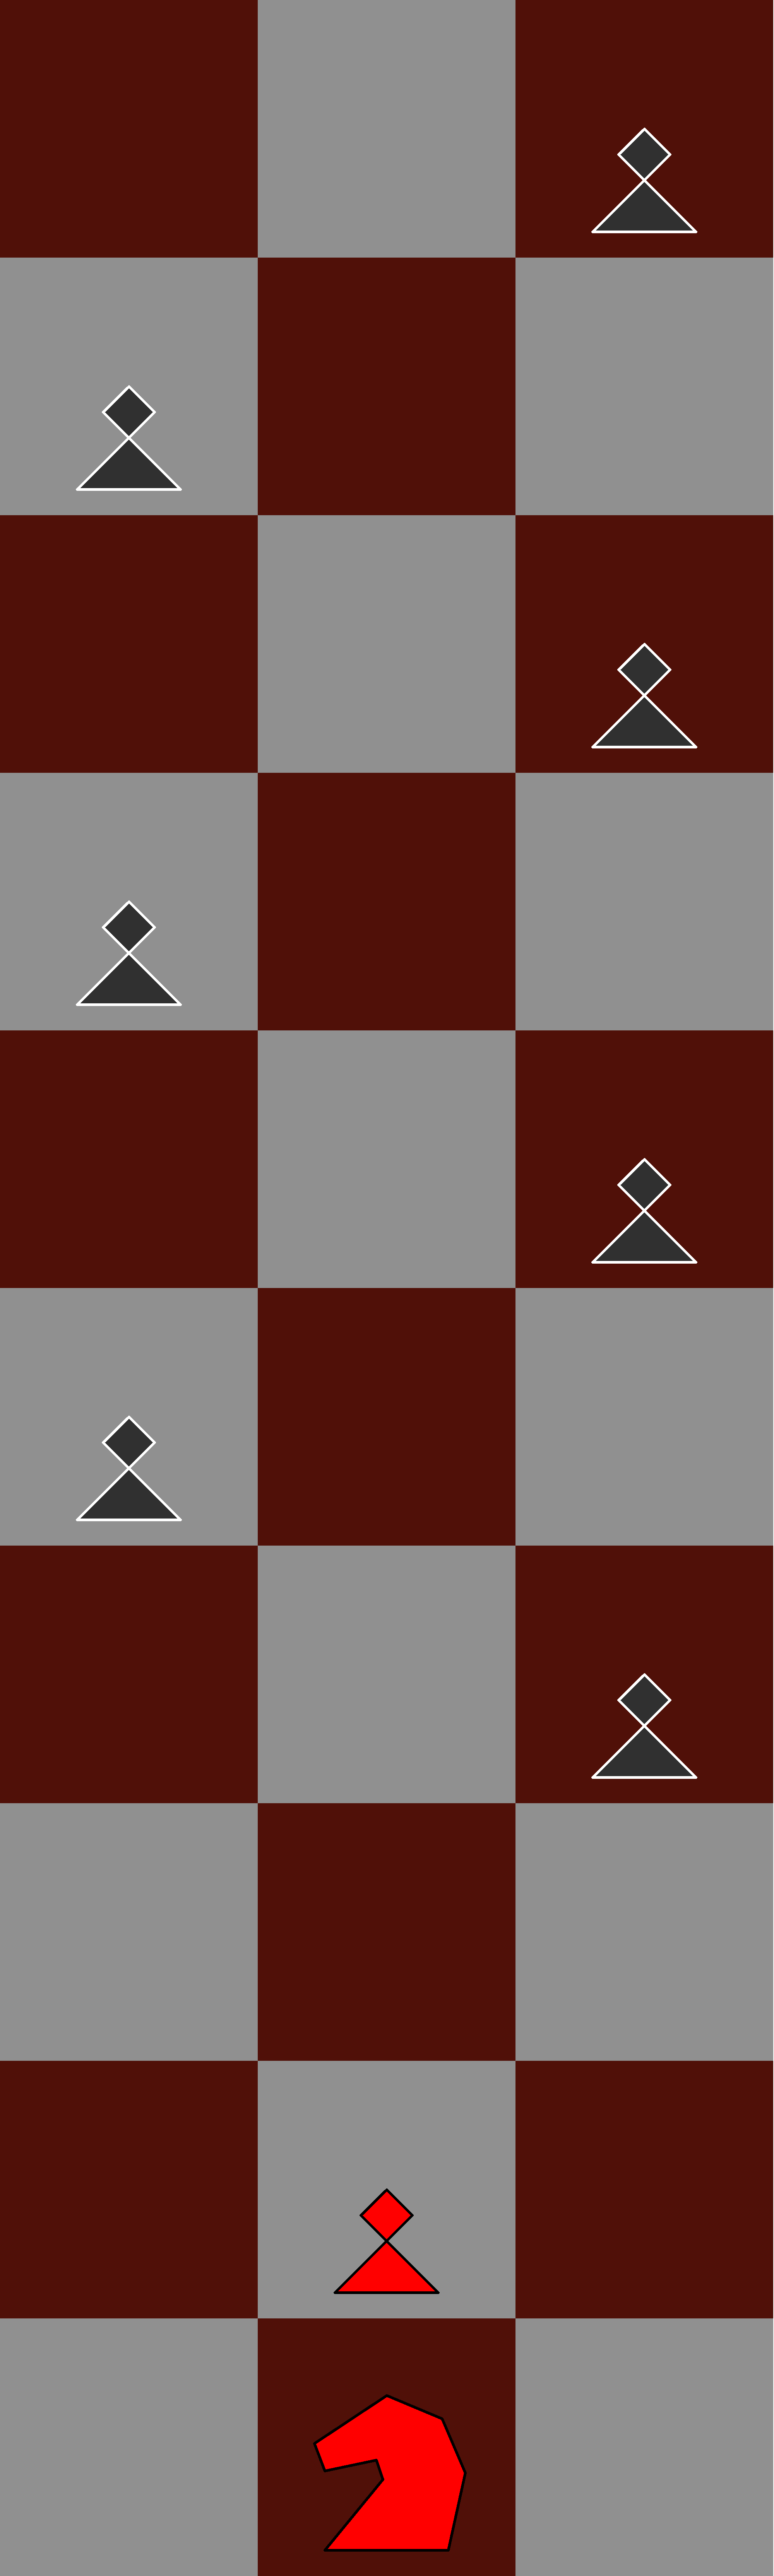
\includegraphics[width=1.0\textwidth, keepaspectratio=true]{en_passants/14_hemera_s_dawn_en_passant.png}
\vspace*{-1.3\baselineskip}
\caption{Rush, en passant}
\label{fig:14_hemera_s_dawn_en_passant}
\end{figure}

\vspace*{-0.5\baselineskip}
Image above have 6 examples presented in parallel: one for each Pawns A, B,
Scouts C, D, and Grenadiers E, F.

Rush and en passant are very similar to those in
\hyperref[fig:12_nineteen_en_passant]{Nineteen variant}.
All privates (Pawns, Scouts, and Grenadiers) can be rushed up to, and including,
the last row on own side of a chessboard. All rushed privates can be captured by
any opponent's private en passant, capturing and captured pieces do not need to
be the same type.

In this variant, Pawns and Grenadiers can be rushed 7 (Pawn A, Grenadier E) or 8
(Pawn B, Grenadier F) fields, depending if they were in first or second privates
row. Scouts can be rushed 5 (Scout C) or 6 (Scout D) fields, depending how close
their starting position is to opponent.

Note, first move of a private (any of Pawns, Scouts, and Grenadiers) is always a
rush, if it moves for 2 or more fields forward, regardless of its normal movement
limits. \newline
\indent
For instance, Scouts in this variant can move at most 5 fields forward; outermost
Scouts could reach end of own side of chessboard without rushing. Regardless, first
move of any Scout from its initial position is a rush, and expose it to possible
capture by en passant, if it moves for 2 or more fields forward.

Converted opponent's privates cannot be rushed, even if converted on initial
positions of own privates.

% \clearpage % ..........................................................

\section*{Promotion}
\addcontentsline{toc}{section}{Promotion}
\label{sec:Hemera's Dawn/Promotion}

Promotion is non enforced, delayed variety, i.e. it's the same as in
\hyperref[sec:Age of Aquarius/Promotion]{previous chess variant}, Age of Aquarius.

Promotion in this variant is polygamous, more than one Queen in the same color
can be present on chessboard at any given time.

\clearpage % ..........................................................

\section*{Castling}
\addcontentsline{toc}{section}{Castling}
\label{sec:Hemera's Dawn/Castling}

Castling is
\hyperref[sec:Nineteen/Castling]{the same as in Nineteen variant},
only difference is that King can move
between 2 and 7 fields across. All other constraints from Nineteen variant still
applies.

\noindent
\begin{figure}[!h]
\includegraphics[width=1.0\textwidth, keepaspectratio=true]{castlings/14_hd/hemera_s_dawn_castling.png}
\caption{Castling}
\label{fig:hemera_s_dawn_castling}
\end{figure}

In example above, all valid King's castling moves are numbered.

\noindent
\begin{figure}[!h]
\includegraphics[width=1.0\textwidth, keepaspectratio=true]{castlings/14_hd/hemera_s_dawn_castling_right_03.png}
\caption{Castling short right}
\label{fig:hemera_s_dawn_castling_right_03}
\end{figure}

In this example King was castling short to the right. Initial King's position is
marked with "K". After castling is finished, right Rook ends up at field immediately
left to the King.

\clearpage % ..........................................................

\section*{Initial setup}
\addcontentsline{toc}{section}{Initial setup}
\label{sec:Hemera's Dawn/Initial setup}

Compared to initial setup of Nineteen, Centaur is inserted between Bishop and Wave
symmetrically, on both sides of chessboard. Scouts are added before first row of Pawns,
and Grenadiers replace some Pawns. This can be seen in the image below:

\noindent
\begin{figure}[h]
\includegraphics[width=1.0\textwidth, keepaspectratio=true]{boards/14_hemera_s_dawn.png}
\caption{Hemera's Dawn board}
\label{fig:14_hemera_s_dawn}
\end{figure}

\clearpage % ..........................................................
% =============================================== Hemera's Dawn chapter
